\section{``Get a Good Ball to Hit''}
In 1971 left-handed hitter Ted Williams published what many baseball players consider a bible of their craft,``The Science of Hitting'' \citep{Williams1971}. In it, Williams credits baseball legend Rogers Hornsby for unsurpassed advice: ``Get a good ball to hit.'' Hornsby meant, and Williams understood, that location makes some pitches easier to hit successfully than others. Williams's famous strike zone visual in Figure 1 encapsulates this advice.\footnote{Please see Appendix A for baseball background and rules; or \citep{Wiki}}
        \begin{figure}[H]
      	\centering
      	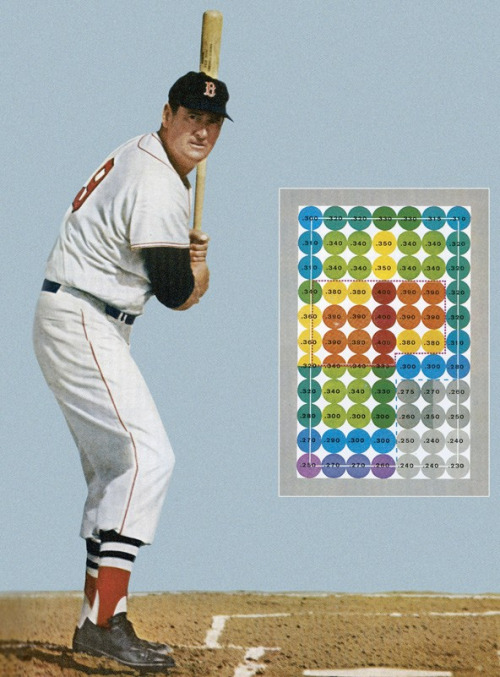
\includegraphics[scale=.35]{Images/Williams.jpg} 
      	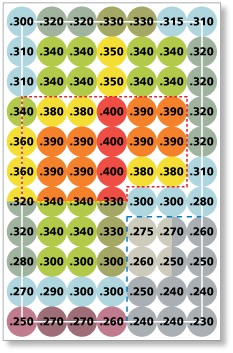
\includegraphics[scale=0.65]{Images/SZ.jpg}
      	\caption{Ted Williams carefully considered which pitch locations he preferred for hitting success. He shows his preferences in this image, where he divided the strike zone into pitch locations with specific probabilities of getting a hit. He labeled the baseballs with personal batting average estimates for pitches in that location \citep{Williams1971}.}
      	\end{figure} 
The strike zone, enlarged on the right, contains baseballs labelled with the batting averages Williams estimated he achieved swinging at pitches in that location. Williams based his estimates on experience and intuition, because no such data existed. In fact, it took another 40 years for technology capable of collecting this type of data to make it to MLB\textsuperscript{\textregistered}.

In 2008 MLB collaborated with a company called Sportsvision, Inc to implement a new technology called PITCHf/x\textsuperscript{\textregistered}. PITCHf/x\textsuperscript{\textregistered} collects the data necessary to analyze, visualize, and model Williams's location-based conception of hitting success.

\section{PITCHf/x\textsuperscript{\textregistered} Data} % ============================================
Sportvision, Inc., based in Chicago, provides the technology to collect PITCHf/x\textsuperscript{\textregistered} data. During the 2007 season Sportvision finished installed three high speed stereoscopic cameras in every MLB\textsuperscript{\textregistered} stadium. Each camera takes approximately 20 images of each pitch in flight and determines its path in three dimensions \citep{Fast2010}. Sportsvision licenses PITCHf/x\textsuperscript{\textregistered} data to Major League Baseball Advanced Media (MLBAM\textsuperscript{\textregistered}) \citep{Baumer2010}. 

        \begin{figure}[H]
      	\centering
      	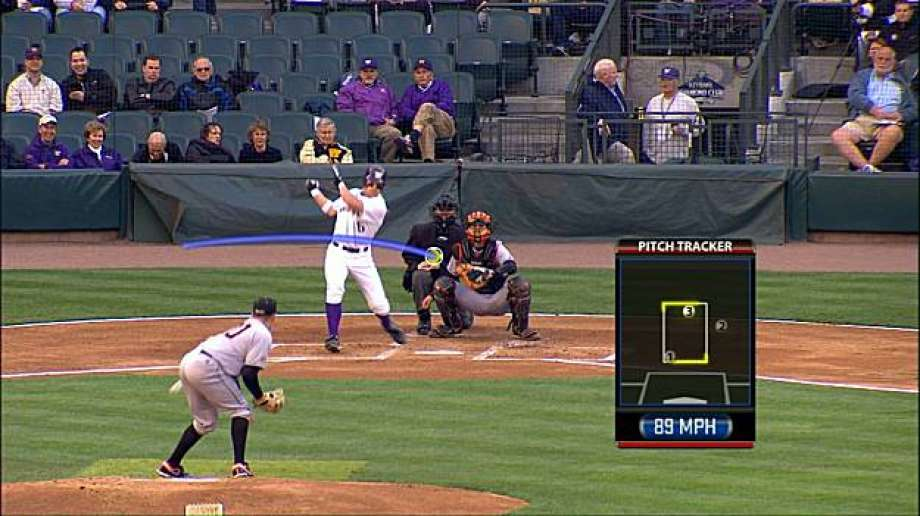
\includegraphics[scale=.4]{Images/PITCHfx.jpg} 
      	\caption{PITCHf/x\textsuperscript{\textregistered} data in your home. Television broadcasts include pitch trajectory and strike zone data, in real time, for the viewer to see.}
      	\end{figure} 
MLBAM\textsuperscript{\textregistered} makes PITCHf/x\textsuperscript{\textregistered} data publicly available online in XML format, calling it ``Gameday'' data \citep{Sievert2014}. A homepage exists for every game, with links organizing data into XML tables with names such as {\it game, inning, at bat, pitch, team, player}, and {\it umpire} \citep{Sievert2014}. The {\it at bat} table, for example, contains data for 15 variables across 1,711,211 at bats. The format and size---on the order of gigabytes---of the data precludes direct download. Instead, XML scripts automate database ready downloads \citep{Adler2006}. We used a MySQL database, and \verb|dplyr| database management functions in R, to manipulate and store 13 PITCHf/x\textsuperscript{\textregistered} tables \citep{Tahaghoghi2006}, \citep{Wickham2016}. 

As an ``in-memory'' application, R uses a computer's limited RAM to host the R environment data \citep{Smith2013}. As a result, data manipulation on this scale requires ``memory management'' techniques \citep{Wickham2014}.  We applied Split-Apply-Combine operations to tables inside the MySQL database, before importing data frames to R \citep{Wickham2011}.

We collected the variables relevant for this research primarily from the {\it at bat} and {\it pitches} tables. We list these variables, with a short description, below \citep{Fast2007}.
  \begin{description}[leftmargin=1.5cm, style=nextline]
  \item[px] location of the pitch on the horizontal axis when it passes through the strike zone (or the extended plane), recorded in feet from the middle of home plate, from the catcher/umpire point of view.
  \item[pz] location of the pitch on the vertical axis when it passes through the strike zone plane, measured in feet above the ground. A negative value implies the ball bounced before reaching home plate
  \item[des] a short description of the outcome of the pitch, i.e. swing and miss, ground ball for out, ground ball for hit, etc.
  \item[id] a unique id for a pitch within a game.
  \item[ab\_id] a unique id for each at bat.
  \item[pitch\_id] a unique identification number for each pitch.
  \item[pitch\_type] a classification of the type of pitch, out of 18 possible types. For example, four seam fastball, two seam fastball, curveball, knuckle ball, etc.
  \item[stand] handedness of the batter, right or left.
  \item[batter] a unique ID for each hitter.
\end{description}

Professional baseball teams, fans, and the baseball media (TV, radio, print, etc)  continually seek more insightful analysis. The collection and distribution of PITCHf/x\textsuperscript{\textregistered} data comes in response to this demand. In the next section we discuss the relevance of statistical analysis of baseball data, and of our research in particular, to these groups.

\section{Baseball Context and Motivation}

Major League Baseball (MLB\textsuperscript{\textregistered}) teams employ approximately 156 quantitative analysts, at a total cost of approximately \$15 million annually \citep{Lindbergh2016}. Teams strive to gain marginal competitive advantages, and analysis of strike zone data provides just this sort of edge, so would generate interest. For example, the heat map in Figure 1.2 indicates right-handed hitters have greater success in the lower one-third of the strike zone than in the top one-third.
        \begin{figure}[H]
      	\centering
      	\includegraphics[scale=.1]{Images/Rudimentary.jpg} 
      	\caption{This simple $5 \times 5$ heat map, explained in much greater detail in Chatper 2 grids, represents the empirical success probability ($\hat{p}_{b}$) of hitter swings at pitches passing through that box.  The data consists of 1,932 right handed hitters, swinging at 1,582,581 pitches between 2008 and 2015.}
      	\end{figure} 
This simple finding contradicts conventional baseball wisdom, which advises pitchers, especially against right-handed hitters, to ``keep the ball down'' \citep{Stallings2003}. A model-based justification for this reversal would generate interest, because teams with this understanding could intelligently target and exploit the misconception. Taken further, if justified in biomechanical terms, biomechanists could analyze the relationship between body types and spatial success probabilities. Then, MLB\textsuperscript{\textregistered} team scouting departments could use this information to more accurately predict hitting success for amateur players of varying builds, a notoriously difficult but lucrative challenge. 

A second example comes at the individual player level. Some MLB\textsuperscript{\textregistered} hitters, such as Joey Votto, have a keen interest in using the most sophisticated analytics available to understand the keys to their success and failure \citep{Daugherty2015}. Votto, who carries a dog-eared copy of Williams's ``The Science of Hitting'' in his bag, pursues such nuances of his craft. The Votto model coefficient estimates could indicate imperceptible strengths and weaknesses to exploit or avoid. 

Regarding media interest, television broadcasts of MLB\textsuperscript{\textregistered} games, such as those on ESPN, TBS, or FOX, regularly integrate PITCHf/x\textsuperscript{\textregistered}-based visuals into the viewing experience \citep{Cross2015}. Figure 1.3 shows a televised baseball graphic made possible by PITCHf/x\textsuperscript{\textregistered}.
        \begin{figure}[H]
      	\centering
      	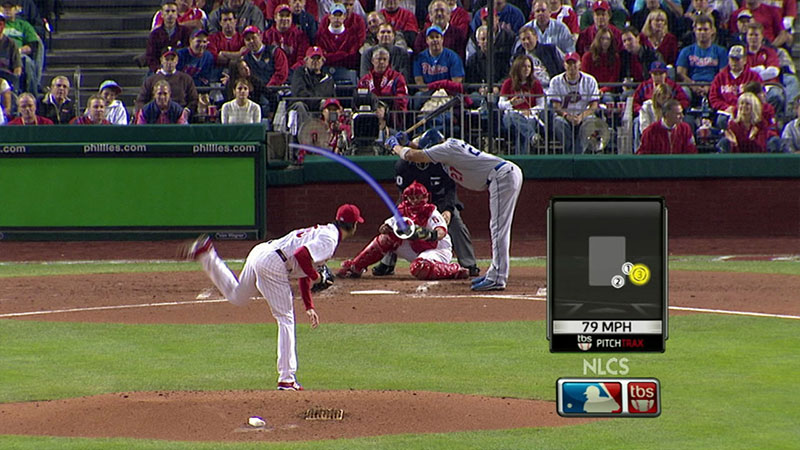
\includegraphics[scale=.4]{Images/PITCHfx2.jpg} 
      	% 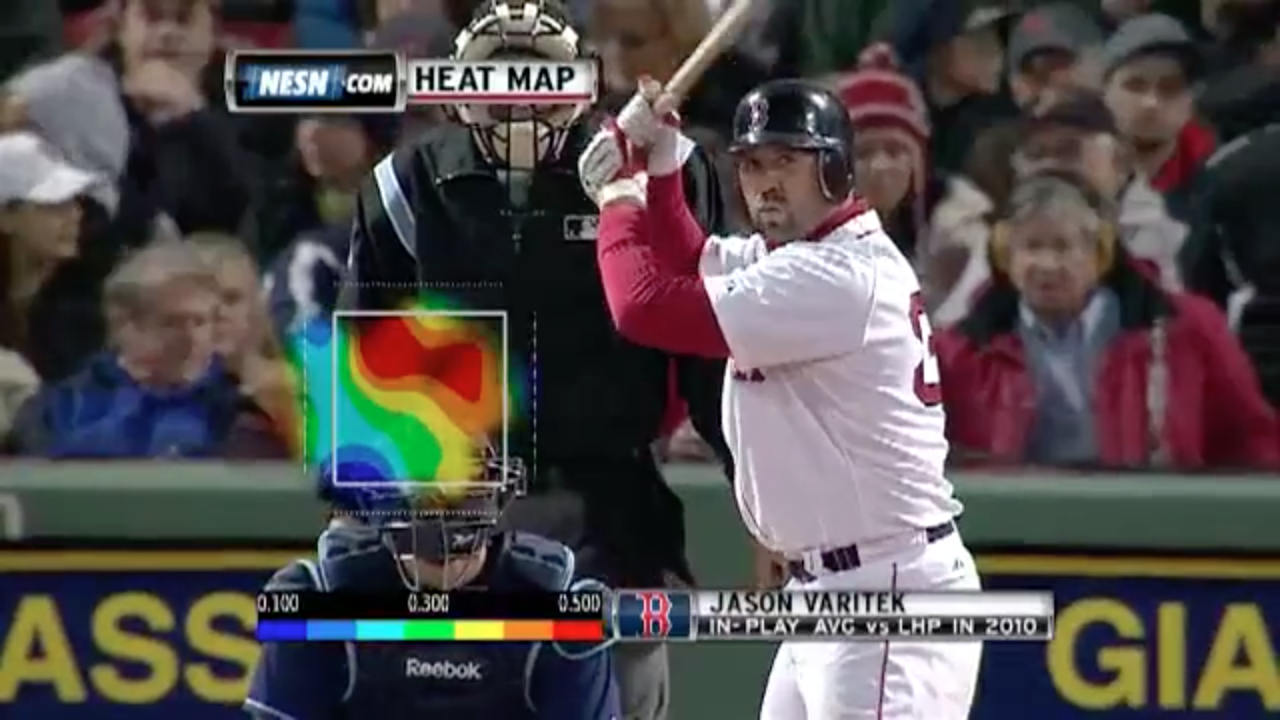
\includegraphics[scale=.25]{Images/Varitek.png} 
      	\caption{PITCHf/x\textsuperscript{\textregistered} data on TV. The graphic shows the pitch's trajectory, and where it passed through the strike zone. The game aired on Turner Broadcast System.} % The lower image includes what appears to be a smoothed empirical heat map on New England Sports Network. We envision an integration of these two visuals.
      	\end{figure} 
This popular type of PITCHf/x\textsuperscript{\textregistered} display appears frequently on MLB\textsuperscript{\textregistered} broadcasts. The image in Figure 1.5, from a game on the New England Sports Network, includes a graphic much less common on TV.
        \begin{figure}[H]
      	\centering
      	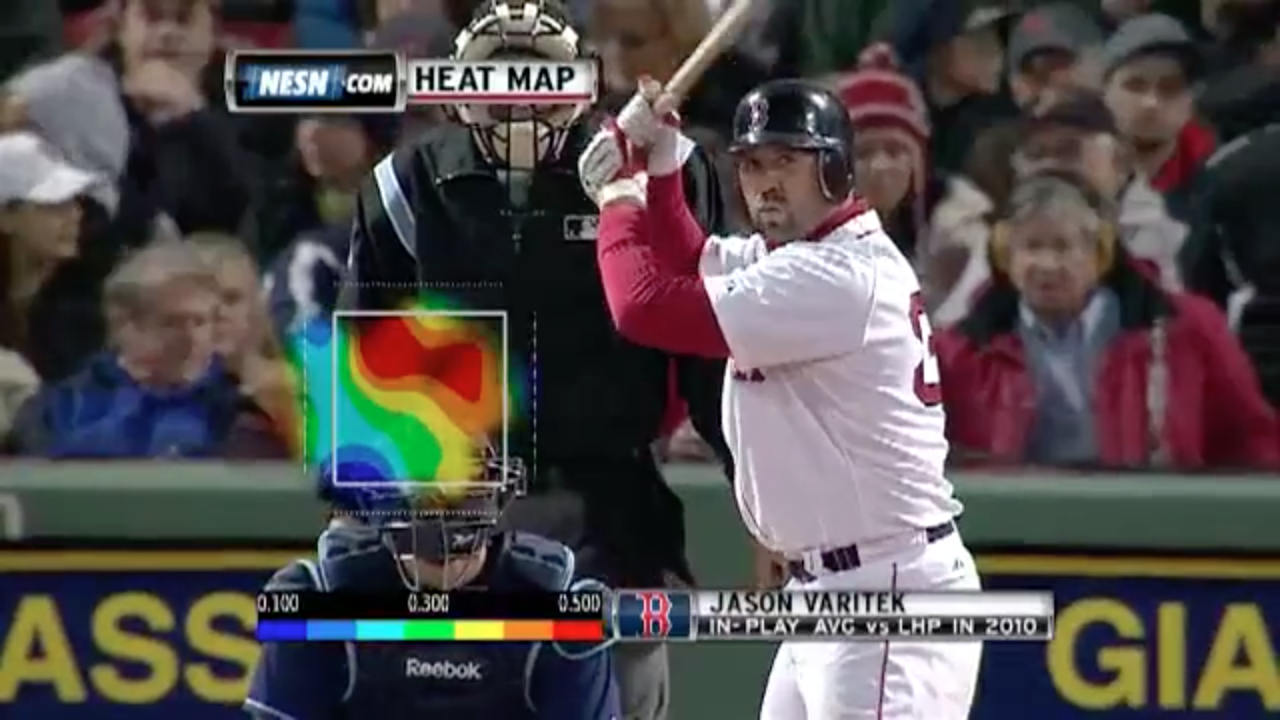
\includegraphics[scale=.25]{Images/Varitek.png} 
      	\caption{PITCHf/x\textsuperscript{\textregistered} data on TV. This image, from a game on the New England Sports Network, includes a smoothed empirical heat map indicating Jason Varitek's spatial success through the strike zone.} 
      	\end{figure} 
The details of this heat map---the data set and statistical techniques used---remain a mystery. Nonetheless, improved visuals serve the interests of MLB\textsuperscript{\textregistered} and the networks; ESPN\textsuperscript{\textregistered} and MLB\textsuperscript{\textregistered} recently agreed to an eight year, \$5.6 billion contract \citep{Newman2012}.

As the dollar amounts suggest, the pursuit of insightful analysis rages on. We are in a unique position, with the requisite expertise and data accessibility, to contribute such insightful analysis. In the next section we describe the preexisting statistical methods and research to provide context for this dissertation.

\section{Statistical Context and Contributions}

% This research includes novel applications of advanced, cutting edge statistical techniques. In addition, as of publication, only one article in a peer reviewed journal focuses on our area of application. This combination---novel application of existing techniques to an unstudied area---constitutes a statistical research contribution. 

We analyze baseball data, but more specifically we analyze strike zone data. As of publication, \cite{Cross2015} constitutes the {\it only} statistical analysis of baseball data in a peer reviewed journal. This surprises, given the widespread enthusiasm for baseball, until considering a few obstacles. First, PITCHf/x\textsuperscript{\textregistered} data collection began relatively recently, in 2008. Second, analysis requires proficiency in statistics, programming, and database management. Third, MLB teams, facing the reality of a zero sum game, conduct research in isolation, and rarely share findings. In sum, these factors help explain the paucity of research. However, our efforts rely on ample previous statistical research, and a some outside of statistics.

Our inspiration to model strike zone success owes Ted Williams a debt, for planting the initial seed with ``The Science of Hitting'' \citep{Williams1971}. As for an intersection of baseball and statistical research, \cite{Cross2015} provides the only peer reviewed literature to use as a starting point. The initial heat map in \cite{Cross2015} intimated---to us---that expressing pitch locations in polar coordinates might help explain spatial variation. 
        \begin{figure}[H]
      	\centering
      	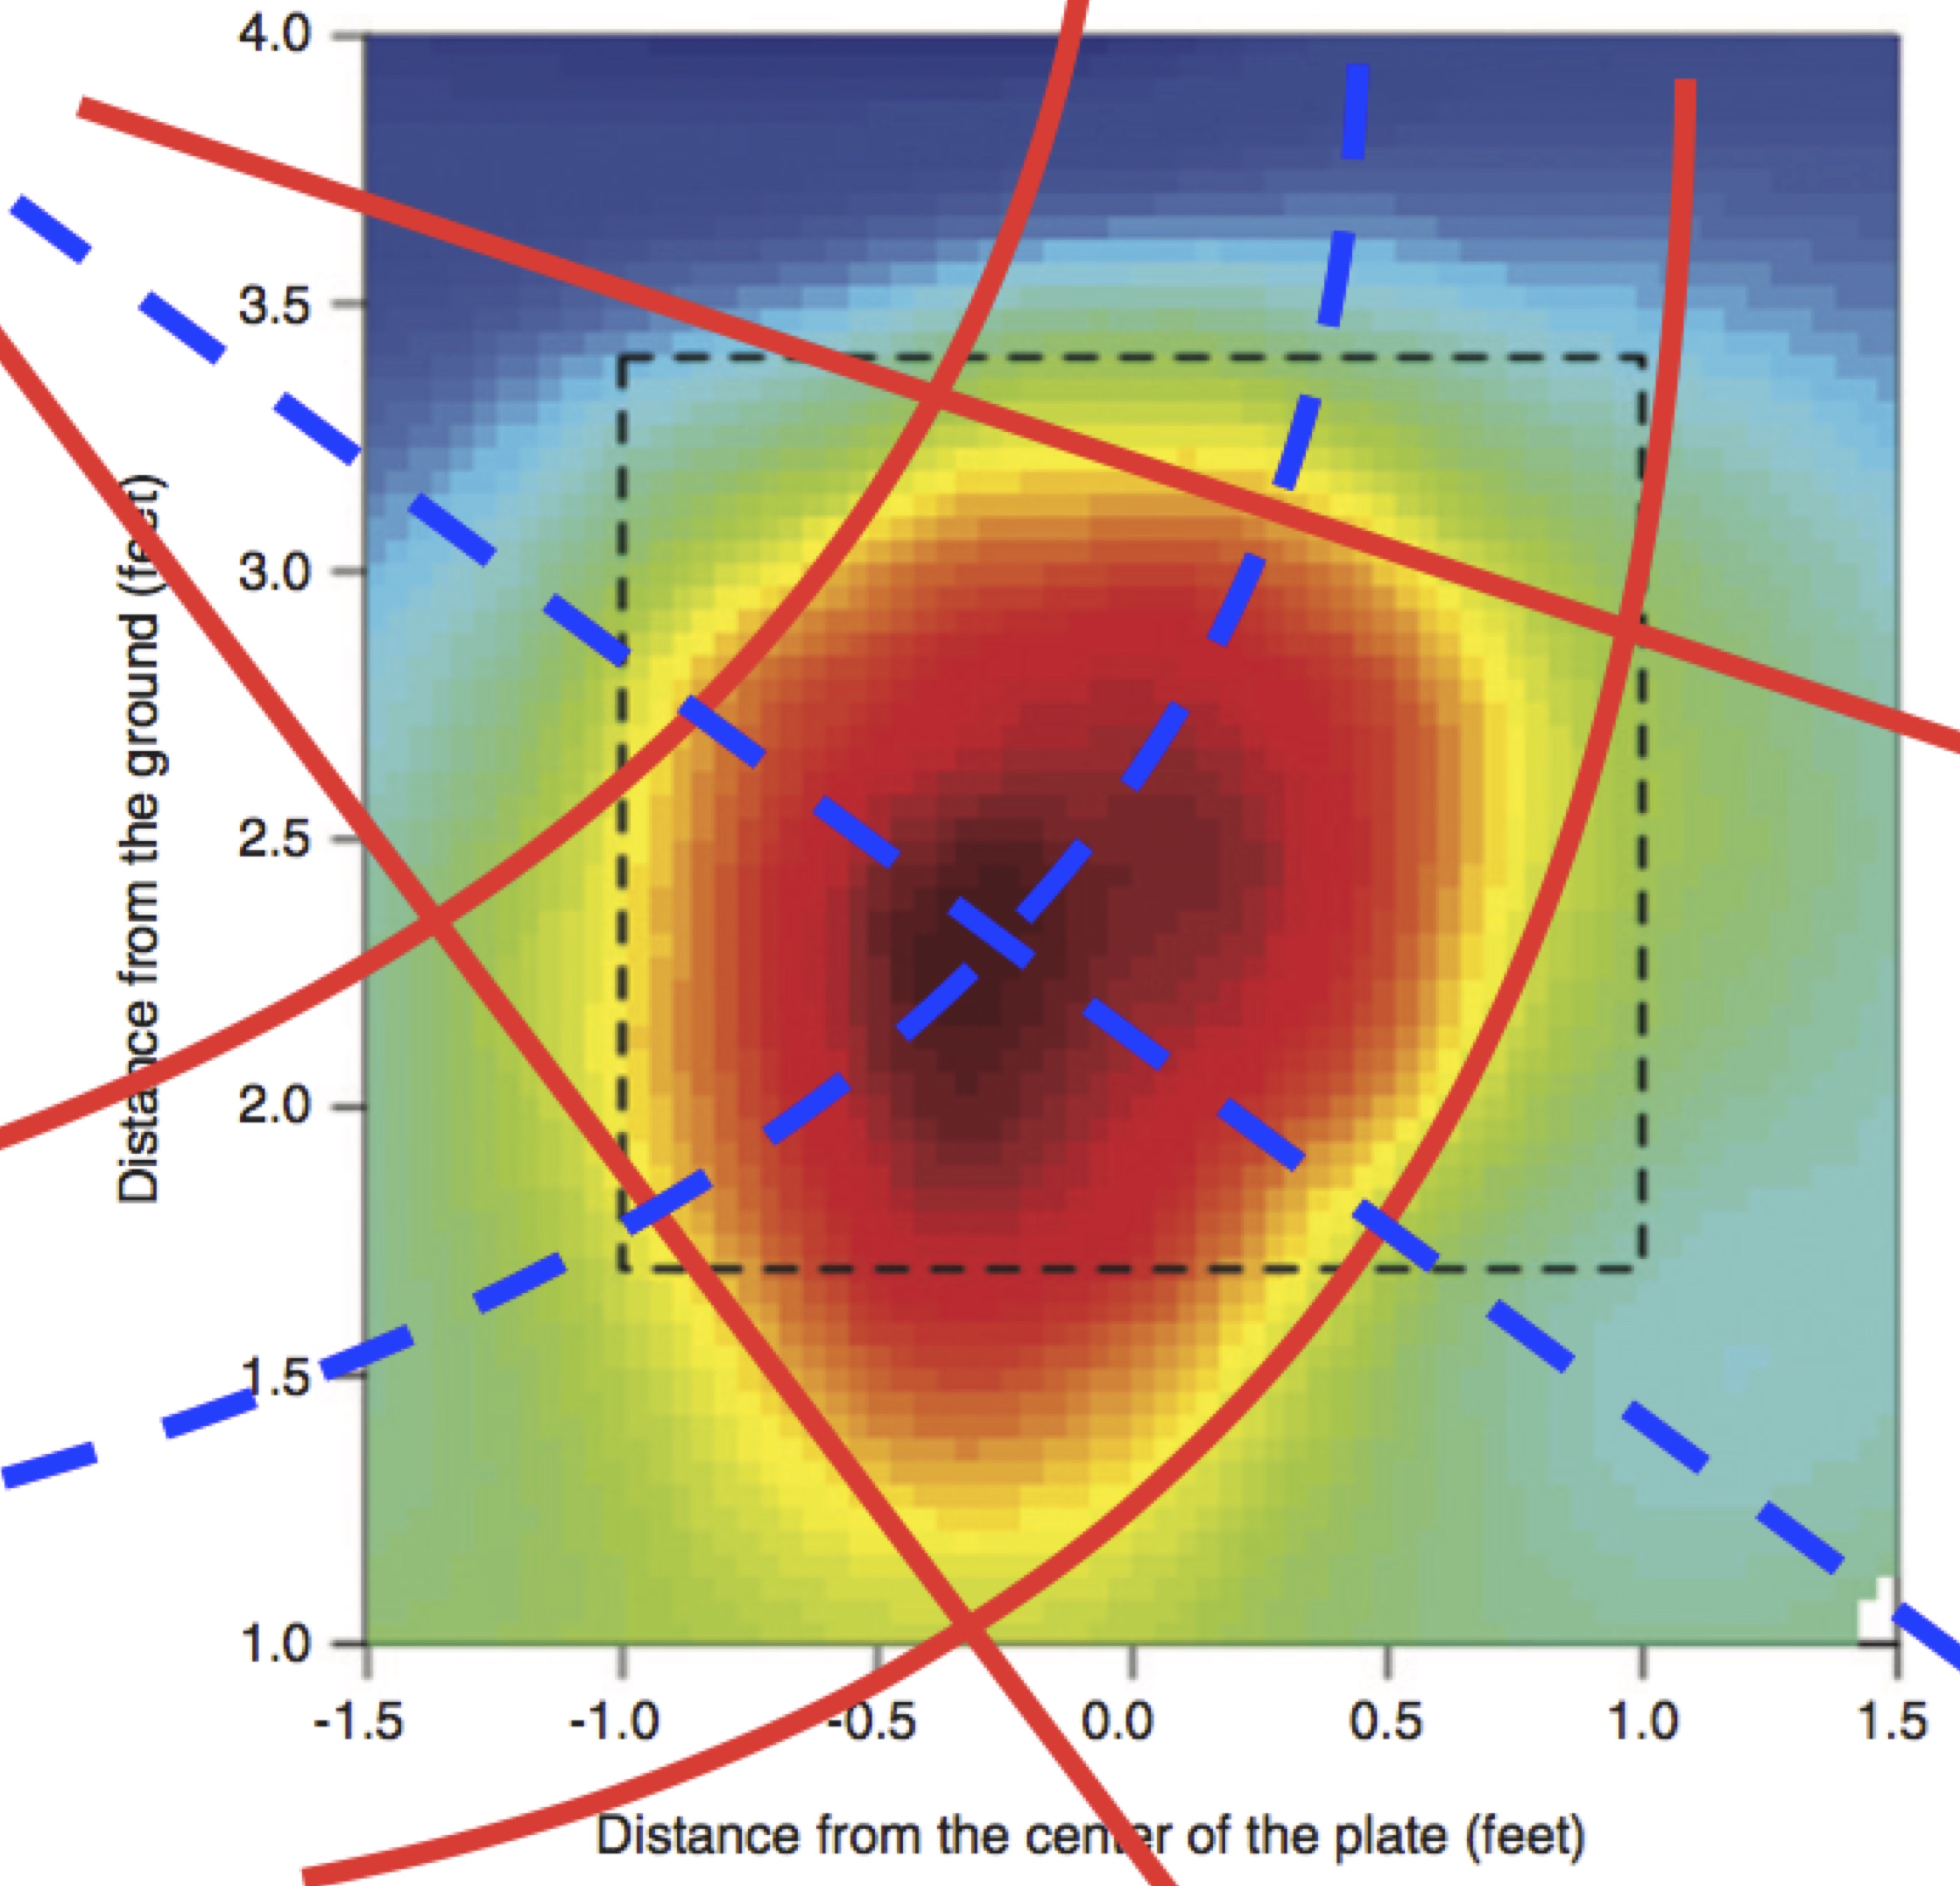
\includegraphics[scale=0.04]{Images/CrossPolar2.jpg} 
      	\caption{\cite{Cross2015} empirical heat map (undisclosed smoothing method). The general shape of the colored region seems to suggest polar coordinates. We added the radial and angular lines to show how we envisioned polar coordinates helping explain spatial variation.}
      	\end{figure}
The added lines in Figure 1.4 depict polar coordinates as we envisioned using them. Notice that expressing pitch locations in polar coordinates involves a translated origin. Conducting research into this non-trivial matter, Glenn Fleisig at the American Sports Medical Institute \citep{Fleisig2002} and Brittany Dowling at Motus \citep{Dowling2016} provided feedback and encouragement. 

In contrast to \cite{Cross2015}, we sought a parametric model; Bernoulli response data suggests a generalized linear model (GLM) with logistic link \citep{Myers2012}. The Hosmer-Lemeshow goodness of fit test validated our polar coordinate based modeling approach \cite{Hosmer2013}. From there, we followed three distinct research paths:
\begin{enumerate}
\item Improving heat map visualizations for our data and analysis, and thus for all spatial data; and 
\item Addressing the $\mathcal{O}(n^{3})$ increase in computational costs incurred for adding a spatial random effect to our model \citep{Finley2009}.
\end{enumerate}
First, heat maps. Impetus for the first innovation comes from empirical heat maps of our data. Hadley Wickham's ``layered grammar of graphics'' in \verb|ggplot2| supplied many of the necessary tools \citep{Wickham2009}, \citep{Wickham2010}; and Doug Nychka's spatial data package \verb|fields| provided critical underlying spatial functions \citep{Nychka}. The second innovation improves the method for presenting heat map confidence intervals. RStudio's ``interactive web application framework'' Shiny provided the dazzling new tools necessary for this innovation \citep{Shiny}.

% --------------- STOPPED HERE ------------------------

Regarding the second path, generally speaking Bayesian hierarchical spatial models accommodate a spatial random effect handily \citep{Gelman2014}, \citep{Banerjee2014}, \citep{Oliver2005}. However, we fit our polar-biomechanical GLM to thousands, and tens of thousands of observations. This created big data challenges, including the "big N" problem. Hadley's \verb|dplyr| proved central to local database management \citep{Wickham2016}. The ``split-apply-combine strategy,'' in tandem with MySQL, provided important data wrangling tools \citep{Wickham2016}, \citep{Tahaghoghi2006}. After initial data wrangling steps, we took three swings at the ``big N'' problem: computational optimization, dimension reduction, and approximation.

We computationally optimized in the Bayesian programming language Stan, with the R interface \verb|rstan| \citep{rstan}, \citep{Gelman2015}. We pored over the manual \citep{STANtheMan}; and Stan developers Andrew Gelman, Rob Trangucci, and Bob Carpenter offered personal assistance \citep{Gelman}, \citep{Trangucci}, \citep{Carpenter}.

The second ``big N'' approach used tools developed by Andrew Finley, professor of Forestry and Geography at Michigan State. Finley helped develop predictive process models, a dimension reduction technique and our second approach \citep{Banerjee2008}, \citep{Finley2012}. Predictive process models craftily reduce computational dimensionality, and we implemented this approach with Finley's package \verb|spBayes| \citep{Finley2013}.

Finally, we tried a cutting edge approximation techniques. The integrated nested Laplace approximation (INLA), a mathematically complex and computationally sophisticated procedure, gives speedy estimates for models with a discrete domain \citep{Rue2009}, \citep{Rue2005}. Therefore, as best practices prescribe, we used a stochastic partial differential equation (SPDE) to modify our model domain to qualify for INLA \citep{Lindgren2011}, \citep{Lindstrom2016}. This exceedingly complex algorithm brings strengths and weaknesses \citep{Mondal2017}, \citep{Simpson2012b}, \citep{Rue2009}.

As this overview demonstrates, our research relied on the contributions of numerous other statisticians, programmers, scientists, and even a baseball player. Next, we lay out how this dissertation proceeds.

\section{Road map}

This dissertation has the following layout. In Chapter 2 we explore the problem of resolution selection for empirical heat maps, especially those with spatially varying data density. We present variable-resolution heat maps, a new option for addressing this problem. Two parts comprise Chapter 3. In the first part we create a generalized linear model for spatial hitter success probabilities, using biomechanical covariates. We manufacture these covariates by expressing pitch locations in the polar coordinate system and strategically translating the polar origin. In the second part, we explain the challenge of heat map confidence intervals, and describe the current, lacking best practices. Therefore, we present an interactive Shiny application solution \citep{Shiny}. In Chapter 4 we add a spatial random effect to the linear predictor in the polar-biomechanical GLM, and deal with the ``big N'' computational consequences. After defining the ``big N'' problem, and we explore three approaches to fitting a ``big N'' spatial generalized linear mixed model. 
